\begin{frame}
    \frametitle{Topics of these slides}
    
    \begin{itemize}
        \item Bayes filter
        \item Kalman filter
        \item Particle filter
    \end{itemize}
    
\end{frame}
    
\begin{frame}
    \frametitle{Localization}
    \begin{block}{Localization}
        It is the ability of a machine (robot) to locate itself in space.
    \end{block}
\end{frame}
    
\begin{frame}
    \frametitle{State Estimation}
    
    \note{Information obtained from Cyrill Stachniss Bayes: https://youtu.be/0lKHFJpaZvE}
    
    \begin{itemize}
        \item Estimate the \textbf{state} $\state$ of a system given the \textbf{observations} $\observation$ and \textbf{control commands} $\controlCommand$
        \item Objective:
    \end{itemize}
    
    \begin{equation}
        p\left(\state_{t} | \observation_{1:t}, \controlCommand_{1:t} \right)
    \end{equation}
    
    Recursive State Estimation: This involves estimating the current state $\state_{t}$ using the immediately preceding state $\state_{t-1}$ as well. \end{frame}
    
    \begin{frame}{Recursive Bayes Filter}
    \begin{block}{Example}
        \begin{itemize}
            \item Given a robot in a one-dimensional world, with no knowledge of where it is
            \item The robot can move forward or backward
            \item Suppose further that there are three doors (\alert{landmarks}), the robot can detect whether it is next to a door or not.
        \end{itemize}
    \end{block}
    
    \begin{center}
        \includegraphics<1>[width=0.7\columnwidth]{./images/monte_carlo_example.pdf}
    \end{center}
    
\end{frame}
    
\begin{frame}
    \frametitle{Recursive Bayes Filter: Initial Position}
    Since the robot initially does not know its position, it is equally possible that it is located anywhere in the world (\alert{belief}). We can represent this mathematically by saying that the robot's \alert{probability distribution function} is \alert{uniform} over the world it is in.
    \begin{center}
        \includegraphics<1>[width=0.7\columnwidth]{./images/monte_carlo_uniform.pdf}
    \end{center}
    
\end{frame}
    
\begin{frame}
    \frametitle{Recursive Bayes Filter: Measurement}
    
    If the robot senses that it is next to a door, then its belief about its location is altered as follows:
    
    \begin{center}
        \includegraphics<1>[width=0.7\columnwidth]{./images/monte_carlo_sensing.pdf}
    \end{center}
    
    This new function represents another probability distribution called \alert{Posterior belief}.
    
    The Posterior belief function is the best representation of the robot's current position. Each hill represents the evaluation of its position relative to a door.
    
    The probability $p(\measurement | \state)$ reads: ``Given that we know where the robot is, what is the probability of observing the door?''
    
\end{frame}
    
\begin{frame}
    \frametitle{Recursive Bayes Filter: Movement}
    
    If \textbf{the robot moves to the right}, the belief changes according to the movement.
    
    Just as the robot's movement is inaccurate, its uncertainty increases as it moves; in other words, the hills are flattened. This flattening is mathematically carried out through the \alert{convolution} operation between the Posterior belief function and the function that describes the distance traveled.
    
    \begin{center}
        \includegraphics<1>[width=0.7\columnwidth]{./images/monte_carlo_moving.pdf}
    \end{center}
    
    The convolution operation measures the overlap as one function slides over another.
    
\end{frame}
    
\begin{frame}
    \frametitle{Recursive Bayes Filter: Second Measurement}
    Suppose the robot, after moving, senses that it is next to a door again. Then, as before, the probability where there is a door will increase by a certain factor of the probability function.
    
    \begin{center}
        \includegraphics<1>[width=0.7\columnwidth]{./images/monte_carlo_sensing2.pdf}
    \end{center}
\end{frame}
    
\begin{frame}
    \frametitle{Recursive Bayes Filter: Second Movement}
    Suppose the robot moves again...
    
    \begin{center}
        \includegraphics<1>[width=0.7\columnwidth]{./images/monte_carlo_moving2.pdf}
    \end{center}
\end{frame}


\begin{frame}
    \frametitle{State Estimation}
    
    \note{Information obtained from Cyrill Stachniss Bayes: https://youtu.be/0lKHFJpaZvE}
    
    \begin{itemize}
        \item Estimate the state $\state$ of a system given the observations $\observation$ and control commands $\controlCommand$
    \item Objective:
    \end{itemize}
    
    \begin{equation}
        p\left(\state_{t} | \observation_{1:t}, \controlCommand_{1:t} \right)
    \end{equation}
    
    Recursive state estimation: This involves estimating the current state $\state_{t}$ using the immediately preceding state $\state_{t-1}$ as well.
\end{frame}
    
\begin{frame}
    \frametitle{State Estimation}
    
    \note{Information obtained from Cyrill Stachniss Bayes: https://youtu.be/0lKHFJpaZvE}
    We are interested in the system's belief (\emph{belief}) about where it is at time $t$:
    
    \begin{equation*}
    bel(\state_{t}) = p\left(\state_{t} | \observation_{1:t}, \controlCommand_{1:t} \right) \quad \text{\scriptsize (state estimation equation or probability distribution definition)}
    \end{equation*}
    
    The equation can be read as: ``Where am I now $\state_{t}$, given all observations $\observation_{1:t}$ and all control commands $\controlCommand_{1:t}$''
    
    \vspace{1cm}
    
    Now let's simplify the distribution using Bayes' Rule:
    
\end{frame}


\begin{frame}
    \frametitle{Derivación del Filtro de Bayes Recursivo}
    
    \note{Información obtenida de Cyrill Stachniss Bayes: https://youtu.be/0lKHFJpaZvE}
    $\begin{aligned}
        \only<1>{
            bel(\state_{t}) &= p\left(\state_{t} | \observation_{1:t}, \controlCommand_{1:t} \right)\\
                }
        \only<2>{
            bel(\state_{t}) &= \alert{p\left(\state_{t} | \observation_{1:t}, \controlCommand_{1:t} \right)}\\
                            &= \eta \, p\left(\observation_{t} |\state_{t}, \observation_{1:t-1}, \controlCommand_{1:t} \right) p\left(\state_{t} | \observation_{1:t-1}, \controlCommand_{1:t} \right) \quad \text{where $\eta$ is a normalization constant}\\
                }
        \only<3>{
            bel(\state_{t}) &= p\left(\state_{t} | \observation_{1:t}, \controlCommand_{1:t} \right)\\
                            &= \eta \, \alert{p\left(\observation_{t} |\state_{t}, \observation_{1:t-1}, \controlCommand_{1:t} \right)} p\left(\state_{t} | \observation_{1:t-1}, \controlCommand_{1:t} \right) \quad \text{where $\eta$ is a normalization constant}\\
                            &= \eta \, p\left(\observation_{t} |\state_{t} \right) p\left(\state_{t} | \observation_{1:t-1}, \controlCommand_{1:t} \right)\\
                }
        \only<4>{
            bel(\state_{t}) &= p\left(\state_{t} | \observation_{1:t}, \controlCommand_{1:t} \right)\\
                            &= \eta \, p\left(\observation_{t} |\state_{t}, \observation_{1:t-1}, \controlCommand_{1:t} \right) p\left(\state_{t} | \observation_{1:t-1}, \controlCommand_{1:t} \right) \quad \text{where $\eta$ is a normalization constant}\\
                            &= \eta \, p\left(\observation_{t} |\state_{t} \right) \alert{p\left(\state_{t} | \observation_{1:t-1}, \controlCommand_{1:t} \right)}\\
                            &= \eta \, p\left(\observation_{t} |\state_{t} \right) \int p\left(\state_{t} | \state_{t-1}, \observation_{1:t-1}, \controlCommand_{1:t} \right) p\left(\state_{t-1} | \observation_{1:t-1}, \controlCommand_{1:t} \right) d \state_{t-1}\\
                }
        \only<5>{
            bel(\state_{t}) &= p\left(\state_{t} | \observation_{1:t}, \controlCommand_{1:t} \right)\\
                            &= \eta \, p\left(\observation_{t} |\state_{t}, \observation_{1:t-1}, \controlCommand_{1:t} \right) p\left(\state_{t} | \observation_{1:t-1}, \controlCommand_{1:t} \right) \quad \text{where $\eta$ is a normalization constant}\\
                            &= \eta \, p\left(\observation_{t} |\state_{t} \right) p\left(\state_{t} | \observation_{1:t-1}, \controlCommand_{1:t} \right)\\
                            &= \eta \, p\left(\observation_{t} |\state_{t} \right) \int \alert{p\left(\state_{t} | \state_{t-1}, \observation_{1:t-1}, \controlCommand_{1:t} \right)} p\left(\state_{t-1} | \observation_{1:t-1}, \controlCommand_{1:t} \right) d \state_{t-1}\\
                            &= \eta \, p\left(\observation_{t} |\state_{t} \right) \int p\left(\state_{t} | \state_{t-1}, \controlCommand_{t} \right) p\left(\state_{t-1} | \observation_{1:t-1}, \controlCommand_{1:t} \right) d \state_{t-1}\\
                }
        \only<6>{
            bel(\state_{t}) &= p\left(\state_{t} | \observation_{1:t}, \controlCommand_{1:t} \right)\\
                            &= \eta \, p\left(\observation_{t} |\state_{t}, \observation_{1:t-1}, \controlCommand_{1:t} \right) p\left(\state_{t} | \observation_{1:t-1}, \controlCommand_{1:t} \right) \quad \text{where $\eta$ is a normalization constant}\\
                            &= \eta \, p\left(\observation_{t} |\state_{t} \right) p\left(\state_{t} | \observation_{1:t-1}, \controlCommand_{1:t} \right)\\
                            &= \eta \, p\left(\observation_{t} |\state_{t} \right) \int p\left(\state_{t} | \state_{t-1}, \observation_{1:t-1}, \controlCommand_{1:t} \right) p\left(\state_{t-1} | \observation_{1:t-1}, \controlCommand_{1:t} \right) d \state_{t-1}\\
                            &= \eta \, p\left(\observation_{t} |\state_{t} \right) \int p\left(\state_{t} | \state_{t-1}, \controlCommand_{t} \right) p\left(\state_{t-1} | \observation_{1:t-1}, \alert{\controlCommand_{1:t}} \right) d \state_{t-1}\\
                            &= \eta \, p\left(\observation_{t} |\state_{t} \right) \int p\left(\state_{t} | \state_{t-1}, \controlCommand_{t} \right) p\left(\state_{t-1} | \observation_{1:t-1}, \controlCommand_{1:t-1} \right) d \state_{t-1}\\
                }
        \only<7>{
            bel(\state_{t}) &= p\left(\state_{t} | \observation_{1:t}, \controlCommand_{1:t} \right)\\
                            &= \eta \, p\left(\observation_{t} |\state_{t}, \observation_{1:t-1}, \controlCommand_{1:t} \right) p\left(\state_{t} | \observation_{1:t-1}, \controlCommand_{1:t} \right) \quad \text{where $\eta$ is a normalization constant}\\
                            &= \eta \, p\left(\observation_{t} |\state_{t} \right) p\left(\state_{t} | \observation_{1:t-1}, \controlCommand_{1:t} \right)\\
                            &= \eta \, p\left(\observation_{t} |\state_{t} \right) \int p\left(\state_{t} | \state_{t-1}, \observation_{1:t-1}, \controlCommand_{1:t} \right) p\left(\state_{t-1} | \observation_{1:t-1}, \controlCommand_{1:t} \right) d \state_{t-1}\\
                            &= \eta \, p\left(\observation_{t} |\state_{t} \right) \int p\left(\state_{t} | \state_{t-1}, \controlCommand_{t} \right) p\left(\state_{t-1} | \observation_{1:t-1}, \controlCommand_{1:t} \right) d \state_{t-1}\\
                            &= \eta \, p\left(\observation_{t} |\state_{t} \right) \int p\left(\state_{t} | \state_{t-1}, \controlCommand_{t} \right) \alert{p\left(\state_{t-1} | \observation_{1:t-1}, \controlCommand_{1:t-1} \right)} d \state_{t-1}\\
                            &= \eta \, p\left(\observation_{t} |\state_{t} \right) \int p\left(\state_{t} | \state_{t-1}, \controlCommand_{t} \right) bel(\state_{t-1}) d \state_{t-1}
                }
    \end{aligned}$
    \only<2>{\alert{Bayes' Rule} \note{eta encodes the normalization performed by the divisor term of Bayes' rule.}}
    \only<3>{\alert{Markov assumption. What I measure now $\observation_{t}$ depends only on the current state $\state_{t}$ and is independent of previous measurements $\observation_{1:t-1}$ and all commands $\controlCommand_{1:t}$}}
    \only<4>{\alert{Law of total probability. That is, we integrate over all possible previous states. This can be interpreted as ``Where are we now, given the previous state $\state_{t-1}$ multiplied by how likely it is that said state $\state_{t-1}$ will be reached.''}}
    \only<5>{\alert{Markov assumption. If $\state_{t-1}$ is given, then all measurements $\observation_{1:t-1}$ and commands $\controlCommand_{t-1}$ are irrelevant. We care about $\controlCommand_{t}$ because it tells us how it evolves from $\state_{t-1}$ to $\state_{t}$ }}
    \only<6>{\alert{Independence assumption. We assume that a future command $\controlCommand_{t}$ does not help us know our current state $\state_{t}$.}} \note{We lose information since we assume independence. We assume that a future command does not help us know our current pose. This is not always true. For example, when a robot is very close to a wall, the control system would hardly give a command that makes the robot move towards the wall. Therefore, if we know that the next command from the control system makes us turn or go backward, then we could infer that we are close to the wall.}
    \only<7>{\alert{Recursive term!}}
    \note{Then we can continue to make assumptions, for example, assuming that the probabilities are Gaussian. Which is not true in general.}
\end{frame}

\begin{frame}{Prediction Step and Correction Step}
    \note{Information obtained from Cyrill Stachniss Bayes: https://youtu.be/0lKHFJpaZvE}
    \begin{itemize}
    \item The Bayes Filter can be written as a two-step process
    \begin{equation*}
    bel(\state_{t}) = \eta \, p\left(\observation_{t} |\state_{t} \right) \int p\left(\state_{t} | \state_{t-1}, \controlCommand_{t} \right) bel(\state_{t-1}) d \state_{t-1}
    \end{equation*}
    \item Prediction Step
    \begin{equation*}
    \overline{bel}(\state_{t}) = \int p\left(\state_{t} | \state_{t-1}, \controlCommand_{t} \right) bel(\state_{t-1}) d \state_{t-1}
    \end{equation*}
    \item Correction Step
    \begin{equation*}
    bel(\state_{t}) = \eta \, p\left(\observation_{t} |\state_{t} \right) \overline{bel}(\state_{t})
    \end{equation*}
    \end{itemize}
    
    \note{The prediction step: predicts where we will be given the control commands}
    \note{The correction step: taking into account the current measurements, corrects the predicted pose}
    
\end{frame}
    
\begin{frame}{Motion model and observation model}
    \note{Information obtained from Cyrill Stachniss Bayes: https://youtu.be/0lKHFJpaZvE} 
    \begin{itemize}
     \item Prediction Step
     \begin{equation*}
     \overline{bel}(\state_{t}) = \int \underbrace{p\left(\state_{t} | \state_{t-1}, \controlCommand_{t} \right)}_{\text{Motion model}} bel(\state_{t-1}) d \state_{t-1}
    \end{equation*}
    \item Correction Step
    \begin{equation*}
    bel(\state_{t}) = \eta \underbrace{p\left(\observation_{t} |\state_{t} \right)}_{\text{\makebox[0pt]{Observation model (Measurement model or Sensor model)}}} \overline{bel}(\state_{t})
    \end{equation*}
    \end{itemize}
    
    \note{The prediction step: predicts where we will be given the control commands}
    \note{The correction step: taking into account the current measurements, corrects the pose predicted}
    
\end{frame}
    
\begin{frame}{Different implementations}
    \note{Information obtained from Cyrill Stachniss Bayes: https://youtu.be/0lKHFJpaZvE}
    \begin{itemize}
    \item The Bayes Filter is a recursive state estimation framework
    \item There are different implementations
    \item Different Properties:
    \begin{itemize}
    \item Linear vs. nonlinear models for motion and observation modeling
    \item Using only Gaussian probability distributions?
    \item Parametric and non-parametric filters (represent the probability distribution parametrically or non-parametrically)
    \item ...
    \end{itemize}
    \end{itemize}
    
\end{frame}
    
\begin{frame}{Popular filters}
    \note{Information obtained from Cyrill Stachniss Bayes: https://youtu.be/0lKHFJpaZvE}
    \begin{itemize}
    \item Kalman Filter
    \begin{itemize}
    \item Uses Gaussian probability distributions
    \item Only works with linear motion and observation models
    \end{itemize}
    \item Extended Kalman Filter (EKF)
    \begin{itemize}
    \item Uses Gaussian probability distributions
    \item {\bf Linearizes} nonlinear motion and observation models using a Taylor approximation
    \end{itemize} 
    \item Particle filter
     \begin{itemize}
     \item Non-parametric
     \item Models of arbitrary probabilistic distributions, that is, not everything is Gaussian (sample sampling stage)
     \end{itemize}
     \end{itemize}
    
     \note{- Nonparametric filters represent posterior state as a function of previous state.
     - Nonparametric filters does not rely on a fixed functional form of
     later.
     - Histogram filter and Particle filter represent state space and posterior as a finite set of data.
     - There is usually a trade-off between efficiency and level of detail of data.}
     \note{the price to pay is that it has a very high computational cost}
    \end{frame}
    
    \begin{frame}{Motion Model}
     \note{Information obtained from Cyrill Stachniss Bayes: https://youtu.be/0lKHFJpaZvE}
     \begin{equation*}
     \overline{bel}(\state_{t}) = \int \underbrace{p\left(\state_{t} | \state_{t-1}, \controlCommand_{t} \right)}_{\text{Motion model}} bel(\state_{t-1}) d \state_{t-1}
     \end{equation*}
\end{frame}

\begin{frame}{Example: Odometry-Based Motion}
    \note{Information obtained from Cyrill Stachniss Bayes: https://youtu.be/0lKHFJpaZvE}
    
    \begin{figure}[!h]
    \centering
    \subfloat[Motion Model Covariance]
    {
    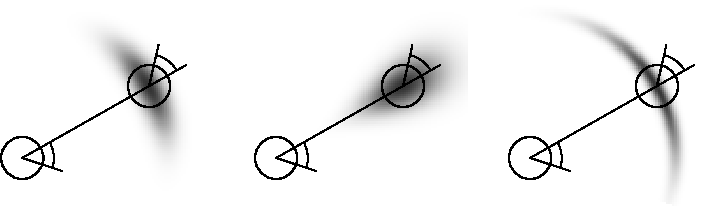
\includegraphics[width=0.6\columnwidth]{./images/covariance_odometry_motion_model.pdf}
    }\\
    \subfloat[Motion Model Samples]
    {
    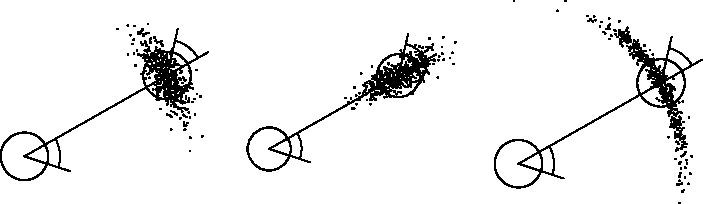
\includegraphics[width=0.6\columnwidth]{./images/sampling_odometry_motion_model.pdf}
    }
    \end{figure}
    
    \end{frame}
    
    \begin{frame}{Observation Model}
    \note{Information obtained from Cyrill Stachniss Bayes: https://youtu.be/0lKHFJpaZvE}
    \begin{equation*}
    bel(\state_{t}) = \eta \underbrace{p\left(\observation_{t} |\state_{t} \right)}_{\text{\makebox[0pt]{Observation model (Measurement model or Sensor model)}}} \overline{bel}(\state_{t})
    \end{equation*}
    \end{frame}
    
    \begin{frame}{Example: Simple Observation Model with Gaussian Noise}
    \note{Information obtained from Cyrill Stachniss Bayes: https://youtu.be/0lKHFJpaZvE}
    
    \begin{itemize}
    \item Range sensor estimating the distance to a nearby object
    \item Gaussian noise in the sensor reading
    \end{itemize} 
    
    \begin{figure}[!h]
        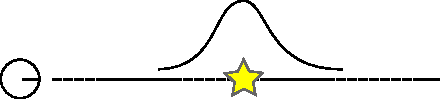
\includegraphics[width=0.6\columnwidth]{./images/simple_observation_model.pdf}
        \end{figure}
    
\end{frame}